% !TeX root = ../main.tex
% Add the above to each chapter to make compiling the PDF easier in some editors.

\chapter{Results}\label{chapter:results}
Based on the thermal profiles which were determined experimentally in \ref{t_prof} the GMPT algorithm will be used to generate schedules for different workloads. Then, for those same workloads, schedules are also derived by the PMPT algorithm \cite{Cheng2015}. These are DPM schedules that also satisfy hard real-time constraints and were calculated by brute force to find the best ratio between the active and inactive CPU state. This produces very accurate data but also requires lengthy computations, resulting in a large overhead. The two approaches will be employed twice, once for a single-task model and once for a multi-task model. The data returned by these experiments will serve to:
\begin{enumerate}[label=(\roman*)]
\item analyze the feasibility of the GMPT algorithm by assessing the performance of its schedules in an environment that closely resembles a typical embedded real-time system.
\item compare the GMPT schedules to another state of the art approach by examining its effect on the thermal development of the processor.
\end{enumerate}
\section{Platform: Notebook}
Two sets of experiments were run on the notebook platform. The first set served to compare the solutions proposed by the two methods within a single-task simulation. In the second set the algorithms tackled a multi-task simulation.
\subsection{Single-Task}
The schedules generated by the two algorithms for 15 different workloads can be seen in \autoref{app:t_pmpt_n} (Appendix). This table clearly demonstrates that the increased effort that is invested in the computation of DVFS schedules doesn't necessarily translate into a more complex schedule. In many cases the schedule derived by GMPT contains only two frequency switches which indicates that the overhead for such schedules won't be much larger than for PMPT schedules (if the frequency setting of the first and last timeslot within a GMPT schedule match, no switch is required between the periods). The thermal behavior of the processor for the GMPT and PMPT schedules is displayed in \autoref{fig:i_eva_gp_n}.\\
\begin{figure}[H]
\begin{subfigure}{.5\textwidth}
  \centering
  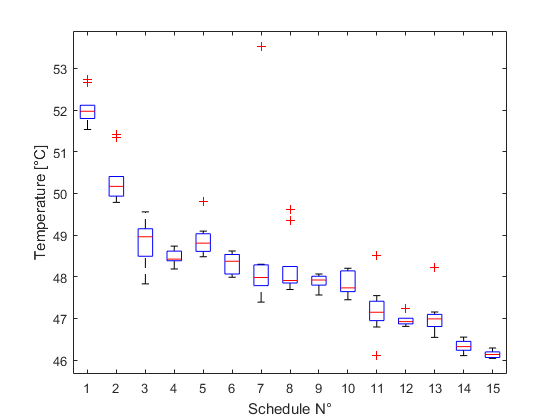
\includegraphics[height=6cm]{figures/eval_gmpt1}
  \caption{Results GMPT}
  \label{fig:i_evg1_n}
\end{subfigure}%
\begin{subfigure}{.5\textwidth}
  \centering
  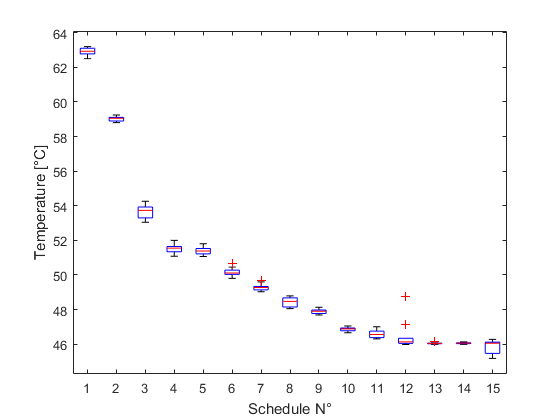
\includegraphics[height=6cm]{figures/eval_pmpt}
  \caption{Results PMPT}
  \label{fig:i_evp_n}
\end{subfigure}
\caption[Results Single-Task Notebook]{Thermal behavior of schedules in single-task environment}
\label{fig:i_eva_gp_n}
\end{figure}
The first few schedules show how a high workload can drastically affect the CPU temperature. Overall both approaches display a similar pattern, naturally struggling with the very high workloads and eventually stabilizing at lower workloads.\\
\hspace*{0.5ex}\hspace{0.5ex} The biggest performance gap between GMPT and PMPT solutions are the high workloads (\autoref{tab:t_medgp_n}). This can be attributed to the cubic influence the frequency/voltage has on the processor power dissipation. Being able to lower the frequency and voltage for a long time period, even if just by a small amount, can have a major impact on the thermal behavior of the platform especially in high frequency ranges. This primarily affects high workloads since in these cases the CPU runs at the maximum frequency for extended periods. This effect is also reflected in the previously computed thermal profile of the notebook.\\
\begin{table}[H]
 \centering
 \caption[Single-Task median results Notebook]{Median peak temperature for all workloads and their performance gap}\label{tab:t_medgp_n}
 \setlength\tabcolsep{5pt}
 \resizebox{\textwidth}{!}{%
 \begin{tabular}{|l||c|c|c|c|c|c|c|c|c|c|c|c|c|c|c|} 
 \hline
  & 1 & 2 & 3 & 4 & 5 & 6 & 7 & 8 & 9 & 10 & 11 & 12 & 13 & 14 & 15 \\ [0.2ex] 
 \hline\hline
 GMPT & 51.9 & 50.1 & 48.9 & 48.4 & 48.8 & 48.3 & 47.9 & 47.9 & 47.9 & 47.7 & 47.1 & 46.9 & 46.9 & 46.3 & 46.1 \\
 \hline
 PMPT & 62.9 & 59 & 53.7 & 51.5 & 51.3 & 50.1 & 49.2 & 48.4 & 47.8 & 46.8 & 46.5 & 46.1 & 46 & 46 & 46 \\
 \hline
 P.Gap & -11 & -8.9 & -4.8 & -3.1 & -2.5 & -1.8 & -1.3 & -0.5 & 0.1 & 0.9 & 0.6 & 0.8 & 0.9 & 0.3 & 0.1 \\
 \hline
\end{tabular}}
\end{table}
Toward lower workloads the difference between the two approaches becomes less clear with the GMPT schedules occasionally resulting in higher peak temperatures. This can, at least in part, be attributed to the increased effectiveness of the idle times due to their longer duration for low workloads. Additionally, with decreasing workloads the peak temperature approaches and converges toward the idle temperature. The performance gap between the two approaches will therefore inevitably shrink. Concerning the accuracy of the measurements \autoref{fig:i_eva_gpbar_n} demonstrates that the spread of data points is very similar for both approaches and that the mean peak temperatures for GMPT and PMPT at low workloads often lie within the spread of each others data points. The performance gap at these workload levels is therefore not considered significant.
\begin{figure}[htpb]
\centering
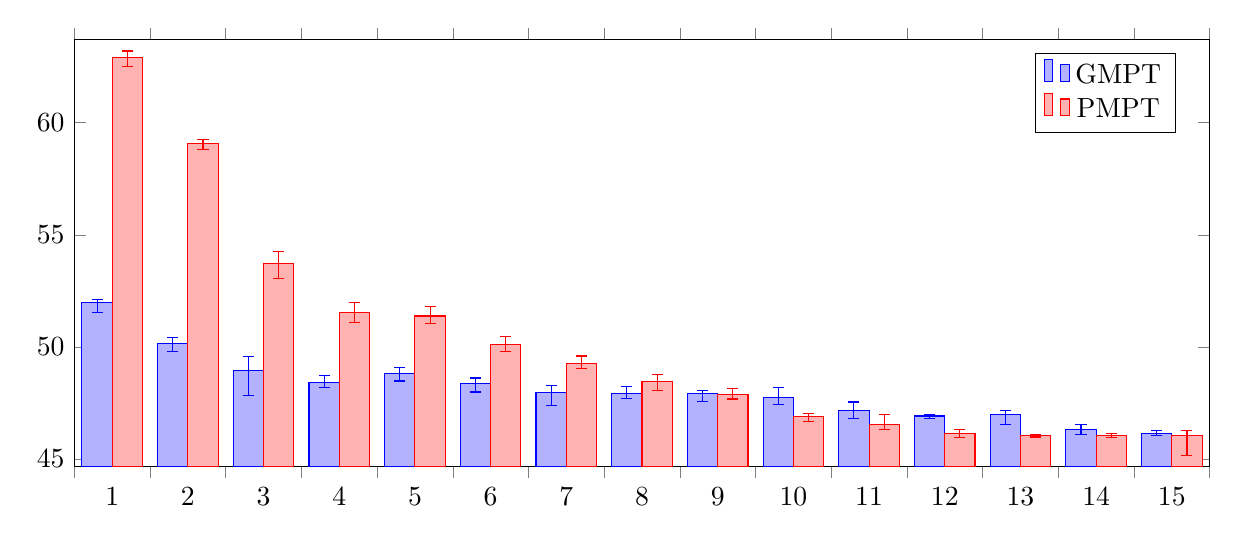
\begin{tikzpicture}
\begin{axis}[
legend pos=north east,
enlargelimits={abs=0.5},
ybar=0pt,
bar width=0.4,
width=16cm,
height=7cm,
xtick={0.5,1.5,...,15.5},
xticklabels={1,...,15},
x tick label as interval
]

\addplot+[error bars/.cd,
y dir=both,y explicit]
coordinates {
    (1,51.9717888360177) += (0,0.141352491928259) -= (0,0.440010384184291)
    (2,50.1668987014317) += (0,0.238370750062352) -= (0,0.383128825312589)
    (3,48.9597483322356) += (0,0.595847508010500) -= (0,1.13150258988060 )
    (4,48.4231287588079) += (0,0.311258328716740) -= (0,0.236621447616535)
    (5,48.8076411054881) += (0,0.285988081180335) -= (0,0.326400991856147)
    (6,48.3728427696685) += (0,0.244936635861023) -= (0,0.383344786044226)
    (7,47.9826060171152) += (0,0.316025495323878) -= (0,0.591076671783732)
    (8,47.9107471809450) += (0,0.333779739462024) -= (0,0.215802033233381)
    (9,47.9206716243684) += (0,0.145610298716868) -= (0,0.358475598043476)
    (10,47.7339920728808) += (0,0.470780310921576) -= (0,0.284585375560390)
    (11,47.1496451599979) += (0,0.396135675248004) -= (0,0.356532442258683)
    (12,46.9225169858525) += (0,0.083227037504123) -= (0,0.114008695210025)
    (13,46.9903069318091) += (0,0.165056482525436) -= (0,0.445691370610206)
    (14,46.3225907340171) += (0,0.229486697802720) -= (0,0.214732313990730)
    (15,46.1342095502068) += (0,0.156640264836348) -= (0,0.093178147706538)};
\addplot+[error bars/.cd,
y dir=both,y explicit]
coordinates {
    (1,62.9278466811292) += (0,0.271521963473894) -= (0,0.427830872232605)
    (2,59.0598958757091) += (0,0.184168050399308) -= (0,0.255963530411819)
    (3,53.7337342397985) += (0,0.525729721145588) -= (0,0.687987842917067)
    (4,51.5474633980814) += (0,0.445812278746146) -= (0,0.467156937429273)
    (5,51.3803222815890) += (0,0.421162669734969) -= (0,0.319064141418743)
    (6,50.1078772800408) += (0,0.345666170336202) -= (0,0.309568791318064)
    (7,49.2719090339404) += (0,0.325140846702602) -= (0,0.243064426806590)
    (8,48.4692716483709) += (0,0.316604304932078) -= (0,0.416873820104783)
    (9,47.8964031221703) += (0,0.232373753015530) -= (0,0.217349072849650)
    (10,46.8824137274556) += (0,0.161036214118710) -= (0,0.226334986945730)
    (11,46.5545351246186) += (0,0.447213228121889) -= (0,0.249776272179105)
    (12,46.1296161091866) += (0,0.208108546541233) -= (0,0.149696036370983)
    (13,46.0413393059249) += (0,0.039757343750920) -= (0,0.056483477251170)
    (14,46.0566087845517) += (0,0.075046329996077) -= (0,0.075049965010769)
    (15,46.0500422026862) += (0,0.226031183493483) -= (0,0.877295127739160)};
\legend{GMPT,PMPT}
\end{axis}
\end{tikzpicture}
\caption[Comparison GMPT PMPT]{Comparison\footnotemark of the temperature measurements for GMPT and PMPT}
\label{fig:i_eva_gpbar_n}
\end{figure}
\footnotetext{The bar values correspond to the median and the error bars correspond to the lower and upper inner fences displayed in the boxplots in \autoref{fig:i_eva_gp_n}}
\subsection{Multi-Task}
The comparison within the multi-task simulation is also based on 15 schedules designed for different workloads, they are reported in \autoref{app:t_ampt_n} (Appendix). Similarly to the previous comparison, many of the GMPT schedules do not require any more frequency switches than the PMPT schedules, diminishing the overhead. \autoref{fig:i_eva_ga_n} depicts the thermal reaction of the notebook platform for the new schedules generated by GMPT and PMPT.\\
\begin{figure}[H]
\begin{subfigure}{.5\textwidth}
  \centering
  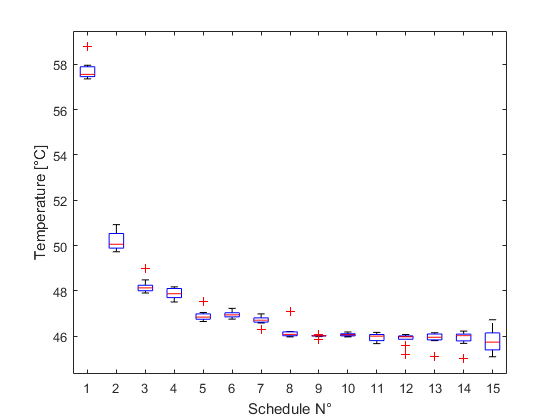
\includegraphics[height=6cm]{figures/eval_gmpt2}
  \caption{Results GMPT}
  \label{fig:i_evg2_n}
\end{subfigure}%
\begin{subfigure}{.5\textwidth}
  \centering
  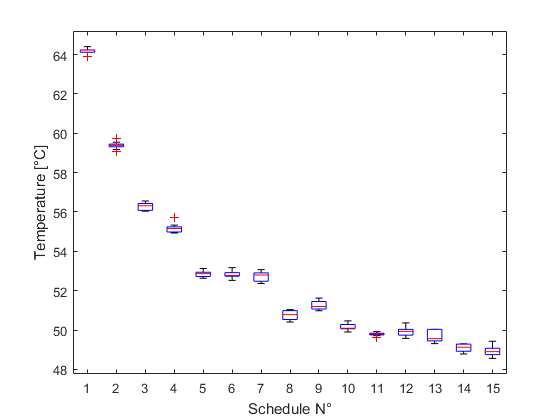
\includegraphics[height=6cm]{figures/eval_ampt}
  \caption{Results PMPT}
  \label{fig:i_eva_n}
\end{subfigure}
\caption[Results Multi-Task Notebook]{Thermal behavior of schedules in multi-task environment}
\label{fig:i_eva_ga_n}
\end{figure}
The overall thermal pattern for both scheduling approaches is again similar, however, contrary to the first comparison, the peak temperature reached by the DPM schedules seem to converge toward a higher temperature level (or at least converge significantly slower). The performance gap for very high workloads is not as big as for the prior comparison but for very low workloads a considerable difference between the two approaches is still visible (\autoref{tab:t_medga_n}).\\
\begin{table}[H]
 \centering
 \caption[Multi-Task Notebook median results]{Median peak temperature for all workloads and their performance gap}\label{tab:t_medga_n}
 \setlength\tabcolsep{5pt}
 \resizebox{\textwidth}{!}{%
 \begin{tabular}{|l||c|c|c|c|c|c|c|c|c|c|c|c|c|c|c|} 
 \hline
  & 1 & 2 & 3 & 4 & 5 & 6 & 7 & 8 & 9 & 10 & 11 & 12 & 13 & 14 & 15 \\ [0.2ex] 
 \hline\hline
 GMPT & 57.5 & 50 & 48.1 & 47.8 & 46.8 & 46.9 & 46.7 & 46 & 46 & 46 & 46 & 45.9 & 45.9 & 46 & 45.7 \\
 \hline
 PMPT & 64.2 & 59.3 & 56.3 & 55.1 & 52.8 & 52.7 & 52.7 & 50.7 & 51.1 & 50 & 49.8 & 49.9 & 49.5 & 49.1 & 48.9 \\
 \hline
 P.Gap & -6.7 & -9.3 & -8.2 & -7.3 & -6 & -5.8 & -6 & -4.7 & -5.1 & -4 & -3.8 & -4 & -3.6 & -3.1 & -3.2 \\
 \hline
\end{tabular}}
\end{table}
The idle temperature of the platform obviously doesn't change depending on the amount of tasks. As visualized in \autoref{fig:i_eva_gabar_n}, the spread of the data points is also too tight to attribute this discrepancy to pure measurement inaccuracies. This phenomenon is probably mostly owed to the fact that a schedule consisting of multiple tasks cannot always be condensed down into one continuous execution block if all tasks run at maximum speed. This means that PMPT must ensure that the active times are sufficiently large to accommodate all tasks. This could lead to situations where during some of the active time, no tasks are running (as they are either finished, haven't been started or cannot start yet). For the GMPT approach this does not constitute a problem since the execution times of each tasks can be "stretched" so that every task finishes as closely as possible to the start of the next task. Under these circumstances GMPT clearly provides the better results from a pure peak temperature minimization standpoint.
\begin{figure}[htpb]
\centering
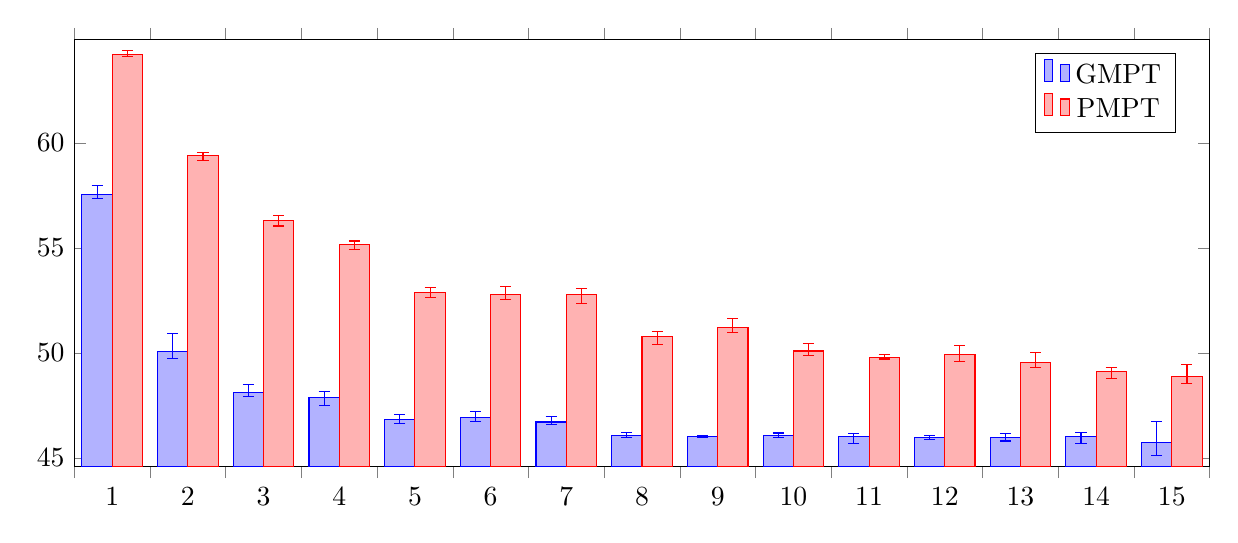
\begin{tikzpicture}
\begin{axis}[
legend pos=north east,
enlargelimits={abs=0.5},
ybar=0pt,
bar width=0.4,
width=16cm,
height=7cm,
xtick={0.5,1.5,...,15.5},
xticklabels={1,...,15},
x tick label as interval
]

\addplot+[error bars/.cd,
y dir=both,y explicit]
coordinates {
    (1,57.5520563450499) += (0,0.398853540814464) -= (0,0.201330990915480)
    (2,50.0604302920827) += (0,0.866091271257638) -= (0,0.331028154367644)
    (3,48.1349022236234) += (0,0.355946483631961) -= (0,0.222823054897276)
    (4,47.8792037719296) += (0,0.303108547127863) -= (0,0.363149943989576)
    (5,46.8457016899354) += (0,0.205369037718071) -= (0,0.189278375646438)
    (6,46.9471570620956) += (0,0.283919388811270) -= (0,0.190102634898516)
    (7,46.7123971085626) += (0,0.278914190099663) -= (0,0.125284290682778)
    (8,46.0886550528459) += (0,0.122945269276471) -= (0,0.111487151874172)
    (9,46.0242732290854) += (0,0.049294756670747) -= (0,0.038824599536404)
    (10,46.0722369733666) += (0,0.118787341594334) -= (0,0.097668077797919)
    (11,46.0081808167382) += (0,0.167245954957863) -= (0,0.330580162767291)
    (12,45.9802630984778) += (0,0.099632234016596) -= (0,0.109006019091346)
    (13,45.9581834222842) += (0,0.202949379069977) -= (0,0.146855052048636)
    (14,46.0288281215878) += (0,0.203512074431124) -= (0,0.337429725415305)
    (15,45.7433702432429) += (0,0.988790539494737) -= (0,0.642572318094373)};
\addplot+[error bars/.cd,
y dir=both,y explicit]
coordinates {
    (1,64.2241375751159) += (0,0.182334478026107) -= (0,0.105106255412579)
    (2,59.3849971691961) += (0,0.160117508425550) -= (0,0.210740141170646)
    (3,56.3173506236765) += (0,0.239900916080224) -= (0,0.274744049470343)
    (4,55.1580628740448) += (0,0.172019951671849) -= (0,0.225918485635077)
    (5,52.8662235798161) += (0,0.262029734087598) -= (0,0.232592431779267)
    (6,52.7709500297011) += (0,0.403868541815093) -= (0,0.244387502709799)
    (7,52.7962794542204) += (0,0.274615958449154) -= (0,0.432018339089105)
    (8,50.7854329474709) += (0,0.251981184023052) -= (0,0.379334349036014)
    (9,51.1949032354764) += (0,0.425712890855209) -= (0,0.215745383261044)
    (10,50.0938467841427) += (0,0.369880420433653) -= (0,0.193792365381015)
    (11,49.8023518920746) += (0,0.118029015092120) -= (0,0.088694652028841)
    (12,49.9302221875302) += (0,0.432539517210600) -= (0,0.355435124434486)
    (13,49.5657769865265) += (0,0.471659460816213) -= (0,0.253872889973046)
    (14,49.1236678371728) += (0,0.180139990117333) -= (0,0.339068851506454)
    (15,48.9006067806866) += (0,0.530949005299846) -= (0,0.342394440693489)};
\legend{GMPT,PMPT}
\end{axis}
\end{tikzpicture}
\caption[Comparison Multi-Task Notebook]{Comparison\footnotemark of the temperature measurements for GMPT and PMPT}
\label{fig:i_eva_gabar_n}
\end{figure}
\footnotetext{The bar values correspond to the median and the error bars correspond to the lower and upper inner fences displayed in the boxplots in \autoref{fig:i_eva_ga_n}}
\section{Platform: Raspberry Pi 3B}
On the Raspberry Pi platform the GMPT and PMPT algorithms were again applied to calculate schedules for single- and multi-task simulations.
\subsection{Single-Task}
The schedules generated by GMPT and PMPT for the different workloads in the single-task environment can be seen in \autoref{app:t_smpt_pi} (Appendix). Even though it is not as pronounced as on the notebook platform, some of the schedules that were computed by the genetic algorithm also require only few frequency changes. For these schedules the influence of the overhead is expected to be very similar for both approaches. However, overall the schedules for the Raspberry Pi do seem to require more frequency changes than those on used on the Notebook. This can at least in part be attributed to the smaller temperature range available on this platform, which likely makes it more difficult to determine which frequency is best at any given point in time.\\
\begin{figure}[H]
\begin{subfigure}{.5\textwidth}
  \centering
  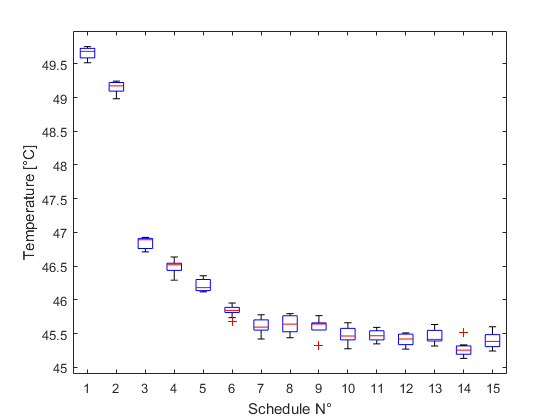
\includegraphics[height=6cm]{figures/gmpt_s_pi}
  \caption{Results GMPT}
  \label{fig:i_evgs_pi}
\end{subfigure}%
\begin{subfigure}{.5\textwidth}
  \centering
  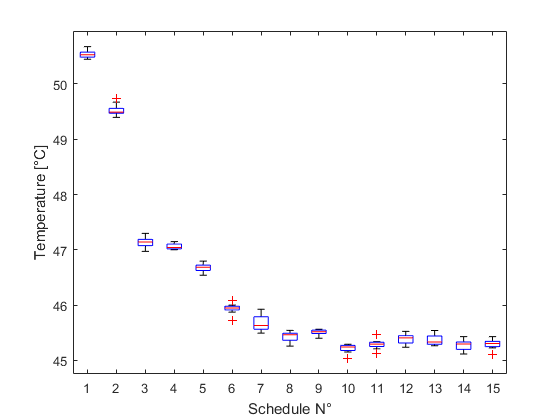
\includegraphics[height=6cm]{figures/pmpt_s_pi}
  \caption{Results PMPT}
  \label{fig:i_evps_pi}
\end{subfigure}
\caption[Results Single-Task Raspberry]{Thermal behavior of schedules in single-task environment}
\label{fig:i_eva_gp_s_pi}
\end{figure}
\autoref{fig:i_eva_gp_s_pi} displays the thermal behavior of the Raspberry Pi CPU for the two kinds of schedules. As indicated by the thermal profiles, the changes in temperature are not as large as on the notebook platform but the temperature development through the 15 schedules still resembles a similar pattern.\\
\begin{table}[H]
 \centering
 \caption[Single-Task median results Raspberry]{Median peak temperature for all workloads and their performance gap}\label{tab:t_sedgp_pi}
 \setlength\tabcolsep{5pt}
 \resizebox{\textwidth}{!}{%
 \begin{tabular}{|l||c|c|c|c|c|c|c|c|c|c|c|c|c|c|c|} 
 \hline
  & 1 & 2 & 3 & 4 & 5 & 6 & 7 & 8 & 9 & 10 & 11 & 12 & 13 & 14 & 15 \\ [0.2ex] 
 \hline\hline
GMPT & 49,7 & 49,2 & 46,9 & 46,5 & 46,2 & 45,8 & 45,6 & 45,6 & 45,6 & 45,5 & 45,5 & 45,4 & 45,4 & 45,3 & 45,4 \\
\hline
PMPT & 50,5 & 49,5 & 47,1 & 47,0 & 46,7 & 45,9 & 45,6 & 45,5 & 45,5 & 45,2 & 45,3 & 45,4 & 45,3 & 45,3 & 45,3 \\
\hline
P.Gap & -0,8 & -0,3 & -0,2 & -0,5 & -0,5 & -0,1 & 0,0 & 0,1 & 0,1 & 0,3 & 0,2 & 0,0 & 0,1 & 0,0 & 0,1 \\
\hline
\end{tabular}}
\end{table}
The difference in peak temperature for the two scheduling approaches is much smaller than observed on the notebook platform (\autoref{tab:t_sedgp_pi}). While the small temperature range may contribute to this, the behavior appears to differ from the observations on the other platform. The temperatures achieved by the two algorithms doesn't diverge as strongly, even for the highest workload, the GMPT schedules do not appear to provide a strong benefit. As indicated by \autoref{fig:i_eva_ga_n}, the spread of the data points doesn't differ by a significant amount between the two scheduling approaches. This shows that the frequency changes of the DVFS schedules do not add any instability to the achieved temperature.\\
\hspace*{0.5ex}\hspace{0.5ex} On this platform the benefit of the GMPT schedules isn't as pronounced as it appeared on the notebook. In this single-task simulation the peak temperature achieved for low workloads is, to all intents and purposes, the same for both methods, and even for very high workloads, while there is a difference, it doesn't appear to be very strong.
\begin{figure}[htpb]
\centering
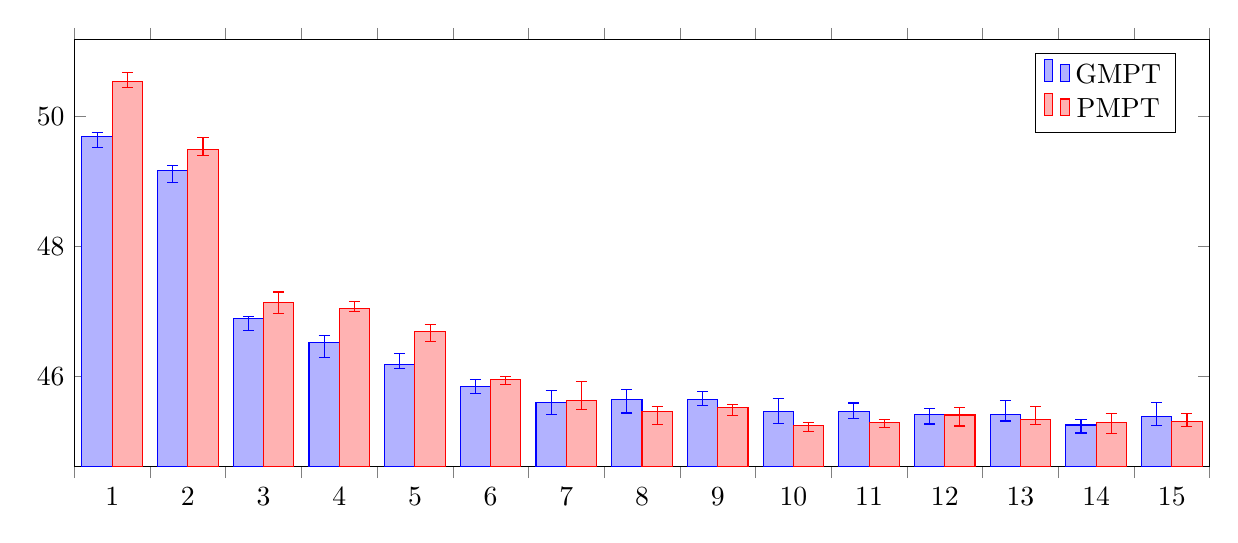
\begin{tikzpicture}
\begin{axis}[
legend pos=north east,
enlargelimits={abs=0.5},
ybar=0pt,
bar width=0.4,
width=16cm,
height=7cm,
xtick={0.5,1.5,...,15.5},
xticklabels={1,...,15},
x tick label as interval
]

\addplot+[error bars/.cd,
y dir=both,y explicit]
coordinates {
    (1,49.68478405) += (0,0.069966455) -= (0,0.168750135)
    (2,49.17207241) += (0,0.07217512) -= (0,0.19090019)
    (3,46.89177851) += (0,0.03515937) -= (0,0.18068561)
    (4,46.5205421) += (0,0.114861455) -= (0,0.229218385)
    (5,46.18018307) += (0,0.17726574) -= (0,0.06153901)
    (6,45.84314179) += (0,0.11067705) -= (0,0.10658501)
    (7,45.59441339) += (0,0.1838183) -= (0,0.17571021)
    (8,45.63928416) += (0,0.156660595) -= (0,0.201670185)
    (9,45.64222696) += (0,0.123004415) -= (0,0.089043455)
    (10,45.46320787) += (0,0.196236365) -= (0,0.189138275)
    (11,45.4666685) += (0,0.124598495) -= (0,0.119399435)
    (12,45.41869495) += (0,0.091439525) -= (0,0.149864225)
    (13,45.41417376) += (0,0.22016078) -= (0,0.09827707)
    (14,45.25437993) += (0,0.077996965) -= (0,0.123072465)
    (15,45.3839802) += (0,0.216019995) -= (0,0.142294955)};
\addplot+[error bars/.cd,
y dir=both,y explicit]
coordinates {
    (1,50.52727257) += (0,0.147734835) -= (0,0.080893685)
    (2,49.49040623) += (0,0.181165205) -= (0,0.095566265)
    (3,47.14078462) += (0,0.156947985) -= (0,0.168154885)
    (4,47.04225844) += (0,0.10671934) -= (0,0.0404122)
    (5,46.68459193) += (0,0.112148575) -= (0,0.143971945)
    (6,45.94851141) += (0,0.052713495) -= (0,0.074132765)
    (7,45.63239278) += (0,0.293799865) -= (0,0.139357765)
    (8,45.46463671) += (0,0.079556745) -= (0,0.206081505)
    (9,45.51780834) += (0,0.046734285) -= (0,0.116654175)
    (10,45.24352346) += (0,0.0486116) -= (0,0.09059746)
    (11,45.29471239) += (0,0.045160185) -= (0,0.084330065)
    (12,45.40729075) += (0,0.119223745) -= (0,0.169417925)
    (13,45.3325583) += (0,0.208028515) -= (0,0.066516575)
    (14,45.29665749) += (0,0.13401067) -= (0,0.17934347)
    (15,45.30736255) += (0,0.123567815) -= (0,0.081026515)};
\legend{GMPT,PMPT}
\end{axis}
\end{tikzpicture}
\caption[Comparison Single-Task Raspberry]{Comparison\footnotemark of the temperature measurements for GMPT and PMPT}
\label{fig:i_eva_sabar_pi}
\end{figure}
\footnotetext{The bar values correspond to the median and the error bars correspond to the lower and upper inner fences displayed in the boxplots in \autoref{fig:i_eva_sabar_pi}}
\subsection{Multi-Task}
In the multi-task environment on the Raspberry Pi the GMPT schedules are the most complex (\autoref{app:t_mmpt_pi}). They require more frequency changes than those under any of the previous conditions. Based on previous observations, this behavior can partly be traced back to the smaller available frequency and temperature range inherent to the platform in combination with the increased challenge of scheduling multiple tasks.\\
\hspace*{0.5ex}\hspace{0.5ex} As illustrated by \autoref{fig:i_eva_gp_m_pi} the temperature development over different workloads follows the familiar pattern observed in previous experiments. The peak temperatures achieved by both algorithms is similar throughout all workloads with schedules for low workload achieving practically the same temperature for both approaches. Only the highest workloads yield a noticeable difference for the two scheduling methods, however, like in the single-task simulations, the difference between the two struggles to reach even $1^\circ C$ (\autoref{tab:t_medgp_pi}).\\
\hspace*{0.5ex}\hspace{0.5ex} Similarly to the multi-task simulation on the notebook, the peak temperatures for the PMPT schedules appear to converge toward a slightly higher temperature but unlike on the other platform it is not clear if this difference can be considered significant.\\
\begin{figure}[H]
\begin{subfigure}{.5\textwidth}
  \centering
  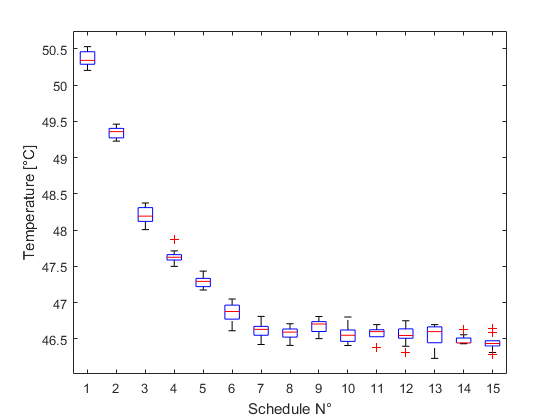
\includegraphics[height=6cm]{figures/gmpt_m_pi}
  \caption{Results GMPT}
  \label{fig:i_evgm_pi}
\end{subfigure}%
\begin{subfigure}{.5\textwidth}
  \centering
  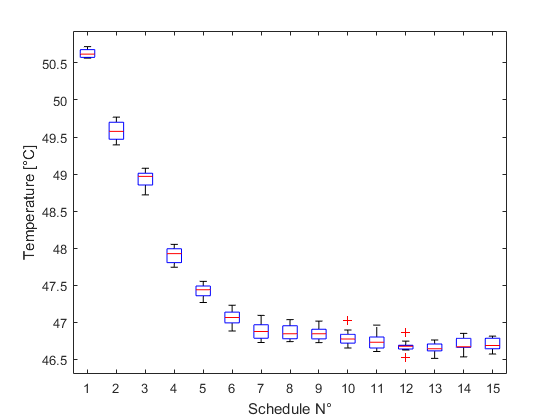
\includegraphics[height=6cm]{figures/pmpt_m_pi}
  \caption{Results PMPT}
  \label{fig:i_evpm_pi}
\end{subfigure}
\caption[Results Multi-Task Raspberry]{Thermal behavior of schedules in multi-task environment}
\label{fig:i_eva_gp_m_pi}
\end{figure}
\begin{table}[H]
 \centering
 \caption[Multi-Task median results Raspberry]{Median peak temperature for all workloads and their performance gap}\label{tab:t_medgp_pi}
 \setlength\tabcolsep{5pt}
 \resizebox{\textwidth}{!}{%
 \begin{tabular}{|l||c|c|c|c|c|c|c|c|c|c|c|c|c|c|c|} 
 \hline
  & 1 & 2 & 3 & 4 & 5 & 6 & 7 & 8 & 9 & 10 & 11 & 12 & 13 & 14 & 15 \\ [0.2ex] 
 \hline\hline
GMPT & 50,3 & 49,4 & 48,2 & 47,6 & 47,3 & 46,9 & 46,6 & 46,6 & 46,7 & 46,5 & 46,6 & 46,5 & 46,6 & 46,4 & 46,4 \\
\hline
PMPT & 50,6 & 49,6 & 49,0 & 47,9 & 47,4 & 47,1 & 46,9 & 46,8 & 46,8 & 46,8 & 46,7 & 46,7 & 46,6 & 46,7 & 46,7 \\
\hline
P.Gap & -0,3 & -0,2 & -0,8 & -0,3 & -0,1 & -0,2 & -0,3 & -0,2 & -0,1 & -0,3 & -0,1 & -0,2 & 0,0 & -0,3 & -0,3 \\
\hline
\end{tabular}}
\end{table}
The comparison provided by \autoref{fig:i_eva_mabar_pi} further shows how close the peak temperatures reached by both scheduling approaches are. For most of the lower workloads the error bars indicate that the difference of the medians is not big enough to clearly demonstrate the behavior observed on the notebook. Regarding the higher workloads, the difference in peak temperature is larger and does demonstrate that the schedules derived by GMPT can provide a benefit under some circumstances. Ultimately, whether the slightly lower temperature for the DVFS schedules justifies their application, considering the increased effort associated with their computation, needs to be evaluated on a case-by-case basis.\\
\hspace*{0.5ex}\hspace{0.5ex} Before drawing a definite conclusion on this platform, the overhead introduced by the framework needs to be taken into account. The analysis in \autoref{chap:ohd_a} has shown, that the frequency changes cause the largest overhead. This mostly affects the DVFS schedules and since it is not clear how highly the CPU is loaded during the execution of the frequency switch, it is not entirely predictable how these lengthy changes affect the temperature development. The results on this platform can therefore not be considered as reliable as the ones from the notebook.
\begin{figure}[H]
\centering
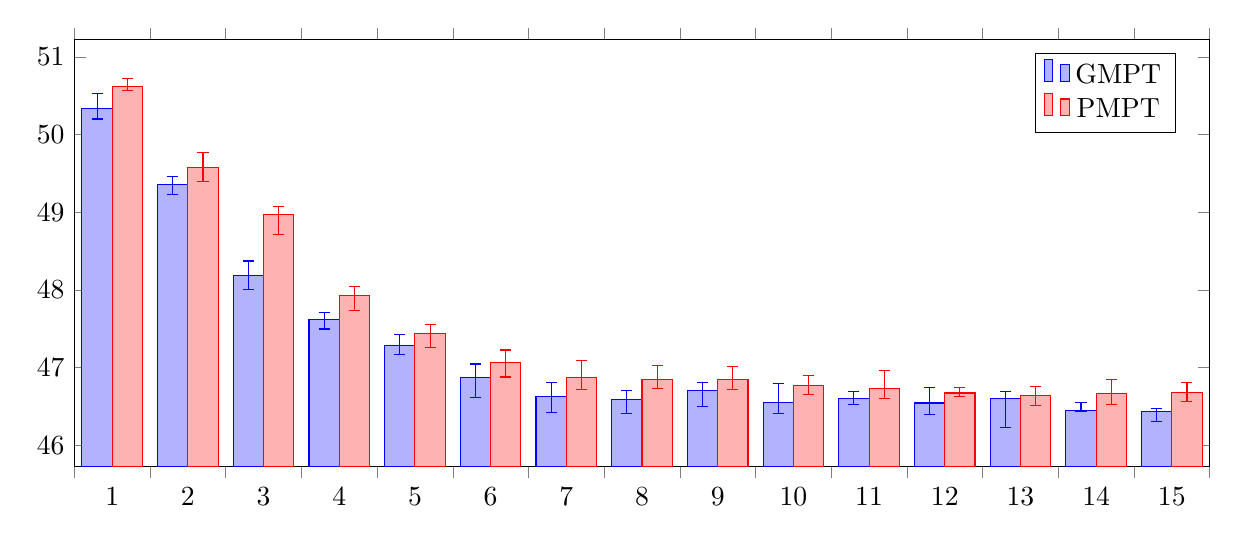
\begin{tikzpicture}
\begin{axis}[
legend pos=north east,
enlargelimits={abs=0.5},
ybar=0pt,
bar width=0.4,
width=16cm,
height=7cm,
xtick={0.5,1.5,...,15.5},
xticklabels={1,...,15},
x tick label as interval
]

\addplot+[error bars/.cd,
y dir=both,y explicit]
coordinates {
    (1,50.33937656) += (0,0.190813545) -= (0,0.137915825)
    (2,49.35669222) += (0,0.104331085) -= (0,0.130885005)
    (3,48.19097365) += (0,0.182186825) -= (0,0.185316615)
    (4,47.62424634) += (0,0.08795757) -= (0,0.12597638)
    (5,47.29060274) += (0,0.141786355) -= (0,0.118604915)
    (6,46.87572704) += (0,0.171886835) -= (0,0.265116815)
    (7,46.62973911) += (0,0.17877497) -= (0,0.20927576)
    (8,46.5920789) += (0,0.114632095) -= (0,0.183715455)
    (9,46.70301373) += (0,0.10315522) -= (0,0.20065271)
    (10,46.54843634) += (0,0.25140397) -= (0,0.14171314)
    (11,46.59903249) += (0,0.09624692) -= (0,0.07110101)
    (12,46.54537319) += (0,0.202520475) -= (0,0.148703605)
    (13,46.59768422) += (0,0.09747961) -= (0,0.36892214)
    (14,46.44280198) += (0,0.112942395) -= (0,0.012193785)
    (15,46.4338047) += (0,0.038619905) -= (0,0.123998935)};
\addplot+[error bars/.cd,
y dir=both,y explicit]
coordinates {
    (1,50.61976356) += (0,0.101523985) -= (0,0.053735465)
    (2,49.57587518) += (0,0.193009565) -= (0,0.181597855)
    (3,48.96792975) += (0,0.109636005) -= (0,0.249692145)
    (4,47.92520965) += (0,0.12491812) -= (0,0.18365727)
    (5,47.43763138) += (0,0.112263245) -= (0,0.173705345)
    (6,47.06281095) += (0,0.165015985) -= (0,0.183683195)
    (7,46.87233309) += (0,0.21922551) -= (0,0.14813599)
    (8,46.84258858) += (0,0.19058075) -= (0,0.10687422)
    (9,46.84206717) += (0,0.171504615) -= (0,0.119597965)
    (10,46.7723845) += (0,0.121608455) -= (0,0.122962645)
    (11,46.72814892) += (0,0.23062294) -= (0,0.12541048)
    (12,46.67324933) += (0,0.06953023) -= (0,0.04985557)
    (13,46.64070392) += (0,0.118115005) -= (0,0.131196595)
    (14,46.66670041) += (0,0.18079879) -= (0,0.13679915)
    (15,46.68468602) += (0,0.12580603) -= (0,0.11506425)};
\legend{GMPT,PMPT}
\end{axis}
\end{tikzpicture}
\caption[Comparison Multi-Task Raspberry]{Comparison\footnotemark of the temperature measurements for GMPT and PMPT}
\label{fig:i_eva_mabar_pi}
\end{figure}
\footnotetext{The bar values correspond to the median and the error bars correspond to the lower and upper inner fences displayed in the boxplots in \autoref{fig:i_eva_mabar_pi}}
\section{Assessment}
Both the single-task and the multi-task simulations have shown that the GMPT algorithm can yield schedules that provide a significant benefit in minimizing the CPU peak temperature, especially for high workloads. The DVFS schedules appear to handle the challenges in multi-task environments especially well when compared to the PMPT solutions (based on evidence provided by the notebook experiments). Here these schedules manage to minimize the peak temperature better than their DPM counterparts throughout all workloads.\\
\hspace*{0.5ex}\hspace{0.5ex} A further factor that could influence the algorithm choice is the time it takes to compute the schedules. The PMPT algorithm is about one order of magnitude faster than the GMPT algorithm. If the schedules are always computed beforehand, this is not an issue, if, however, the static scheduling scheme needs to be adapted at some point during its execution the PMPT approach may be more advantageous.\\
\hspace*{0.5ex}\hspace{0.5ex} The adjustments performed on the notebook and the framework itself succeeded in recreating an environment that resembles a typical hard real-time system. The results provided by the experiments on this platform are therefore considered very reliable and their yields are assumed to be an accurate representation of the performance of both algorithms. The adjustments for the Raspberry Pi on the other hand haven't been as successful. The smaller frequency and temperature range available on this platform makes the comparison of the two approaches undoubtedly more difficult. Additionally, the overhead introduced by the framework is considerably larger than on the notebook, which makes it difficult to draw a clear conclusion regarding the temperature results. Overall the results on this platform cannot be considered as trustworthy as the ones from the notebook. They still provide some evidence that supports the conclusions drawn from the first platform, but when analyzed independently the results are mostly inconclusive.